\documentclass[12pt,a4paper]{article}

\usepackage[a4paper,total={6in,9in}]{geometry}
\usepackage{wrapfig}
\usepackage{graphicx}
\usepackage{amssymb}
\usepackage{mathtools}
\usepackage{listings}
\usepackage{url}
\usepackage{hyperref}
\usepackage{xcolor}
\usepackage{fancyhdr}
\pagestyle{fancy}
\fancyhf{}

\fancyhead[LE,RO]{Latex and Linux}
\fancyhead[RE,LO]{Software Laboratory}
\fancyfoot[CE,CO]{\leftmark}
\fancyfoot[LE,RO]{\thepage}
\renewcommand{\headrulewidth}{2pt}
\renewcommand{\footrulewidth}{1pt}

\hypersetup{colorlinks=true,linkcolor=black,citecolor=red,urlcolor=blue}

\author{\textbf{Abhay Gupta} \\ \textbf{2018EET2555}\\ \textbf{2019-20}}
\date{\today}
\title{\textbf{Assignment-\\ELP- 780 Software  Laboratory}}

\begin{document}
	\maketitle
	
	\begin{center}
	\noindent \large{{A report presented for the assignment on \\ \textbf{Latex and Linux} }}
	\vspace{1cm}
	
	\begin{figure}[h]
	\centering
	
\includegraphics[scale=.2]{iitd.jpg}
	\end{figure}
	\vspace{1.5cm}
	
	\textbf{Departement of Electrical Engineering\\IIT Delhi, India \\ 2019-20}
	
	\end{center}
	
	\newpage
	\tableofcontents
	\listoffigures
	\newpage
	
	\section{Problem Statement}
	
	
		\subsection*{Perform the following actions using commands in Linux terminal only. (30 - 45 minutes)}
		
% 			\begin{enumerate}
% 				\item 
% 				% \item 
% 				% \item 
% 				% \item  
				\begin{itemize}


\item				     Make a new directory in the home folder.
\item Change Directory to this new directory.
\item    Display full path of the Present Working Directory.
 \item   Make a file with .txt extension.
\item    Copy any text of less than 500 words from Wikipedia and paste it in the file.
\item    Change mode of the file to read only.
\item    Display Word Count of the file.
\item    Display number of “the” words in the file using grep command.
\item    Add the sentence “The world is round” to the end of the file, without opening the file.
 \item   Display the last modified time of the file.
\item    Update last modified time of the file to current time, without opening or writing anything to the file.
\item    Create a new empty file without opening the file.
 \item   Copy top 10 lines of the first file to the second file, without opening the file.
 \item   Make a soft link to your Documents directory, in this directory.
  \item  Pipe the command history of terminal to a new file called “terminal.cmd”

								
				\end{itemize}
	\section{Assumptions}
		
			\begin{itemize}
		        \item home \verb+\abhaygupta+ used as home directory.
				\item assumed that terminal works fine.
				\item used ubuntu 18.04
				\item used overleaf for \LaTeX{}
			\end{itemize}
		\subsection{Algorithm and Implementation~\cite{lc}}
		\subsubsection{Commands used }
			\begin{itemize}
				\item mkdir : for making directory
				\item ls : to show files in current directory
			    \item cd : change directory to new directory
			    \item pwd : to see the path of present working directory
			    \item gedit : to create a new file
			    \item chmod : to change access permission to the file
			    \item wc : to get word count of file
			    \item grep : to search and get the word count of specific word
			    \item echo : to add some words at the end of file
			    \item stat : to check the last modified time of file
			    \item touch : to change the modification time to current time and also for make a new file
			    \item sed : to copy some number of lines to other file
			    \item ln : to make a softlink of a directory
			    \item history : to get the history of terminal commands
			\end{itemize}
		
% 		\subsection{Flow Chart}
		
% 			\begin{figure}[h!]
% 				\centering
% 				\caption{Flow Chart for Figure 1}
% 			%	\includegraphics[scale=.6]{}
% 			\end{figure}
		
		\clearpage
		\section{Screenshots}
		
			\begin{figure}[h!]
				\centering
				\caption{Terminal Output}
				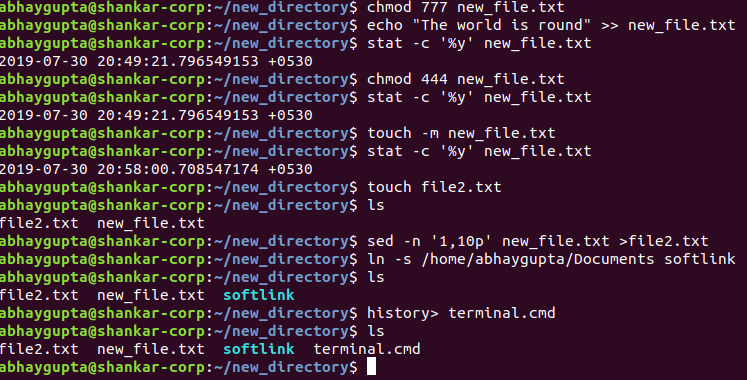
\includegraphics[scale=.5]{2.png}
			\end{figure}
			\begin{figure}[h!]
				\centering
				\caption{Terminal Output}
				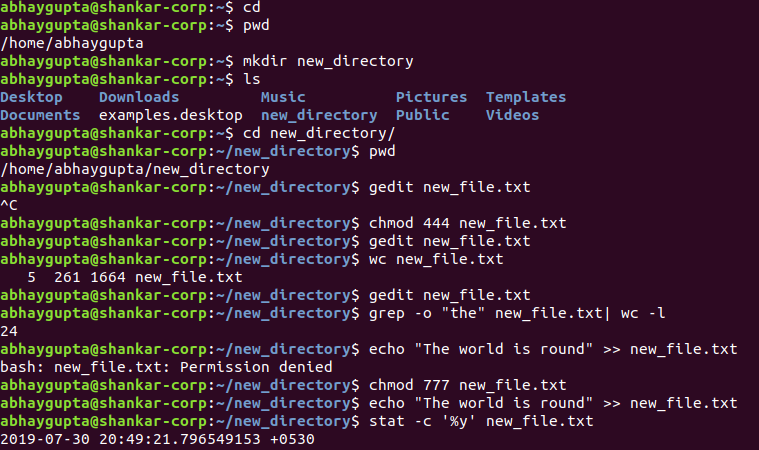
\includegraphics[scale=.5]{1.png}
			\end{figure}
				\begin{figure}[h!]
				\centering
				\caption{\textbf{new\_directory} is created in home directory}
				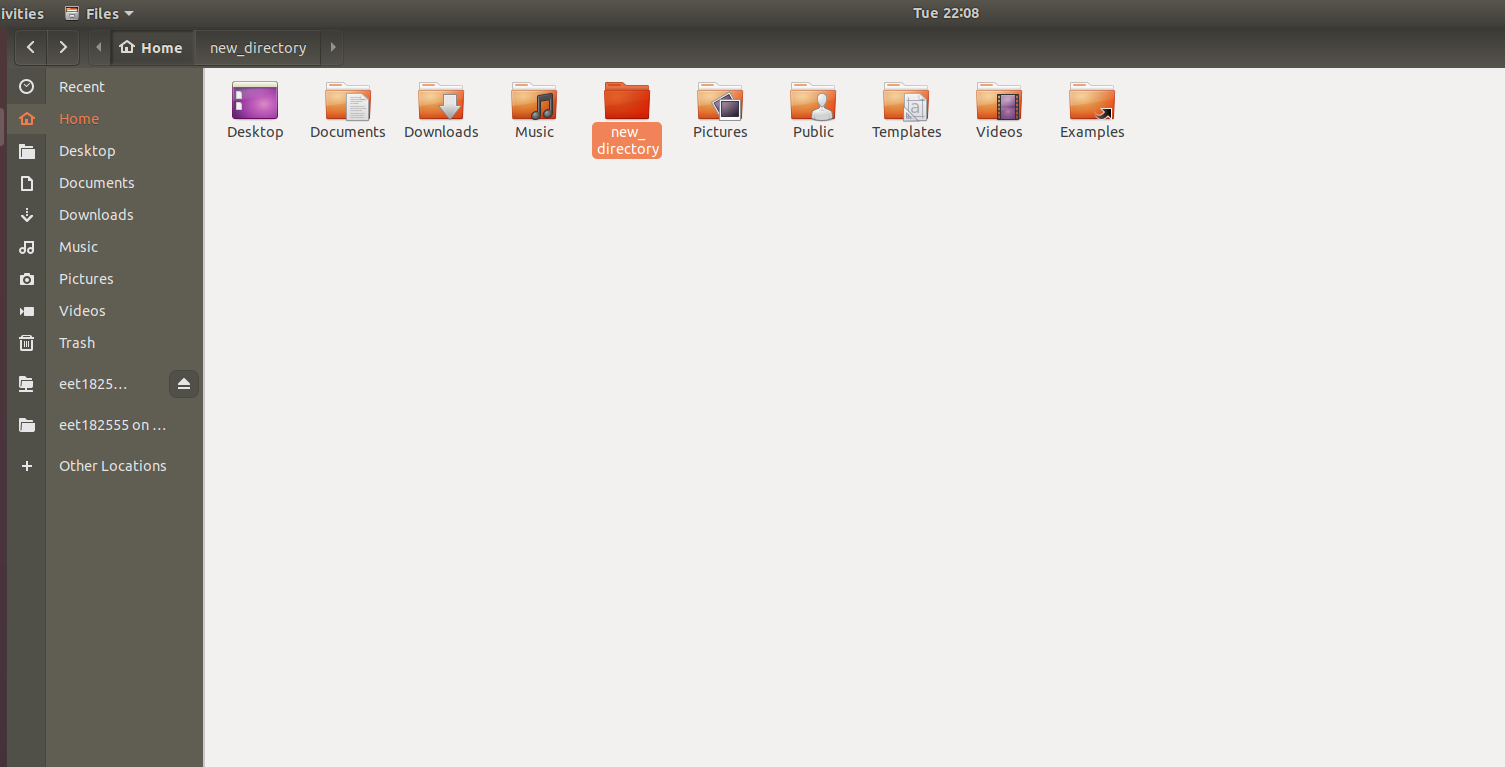
\includegraphics[scale=.25]{home.png}
			\end{figure}
			\begin{figure}[h!]
				\centering
				\caption{files inside new\_directory}
				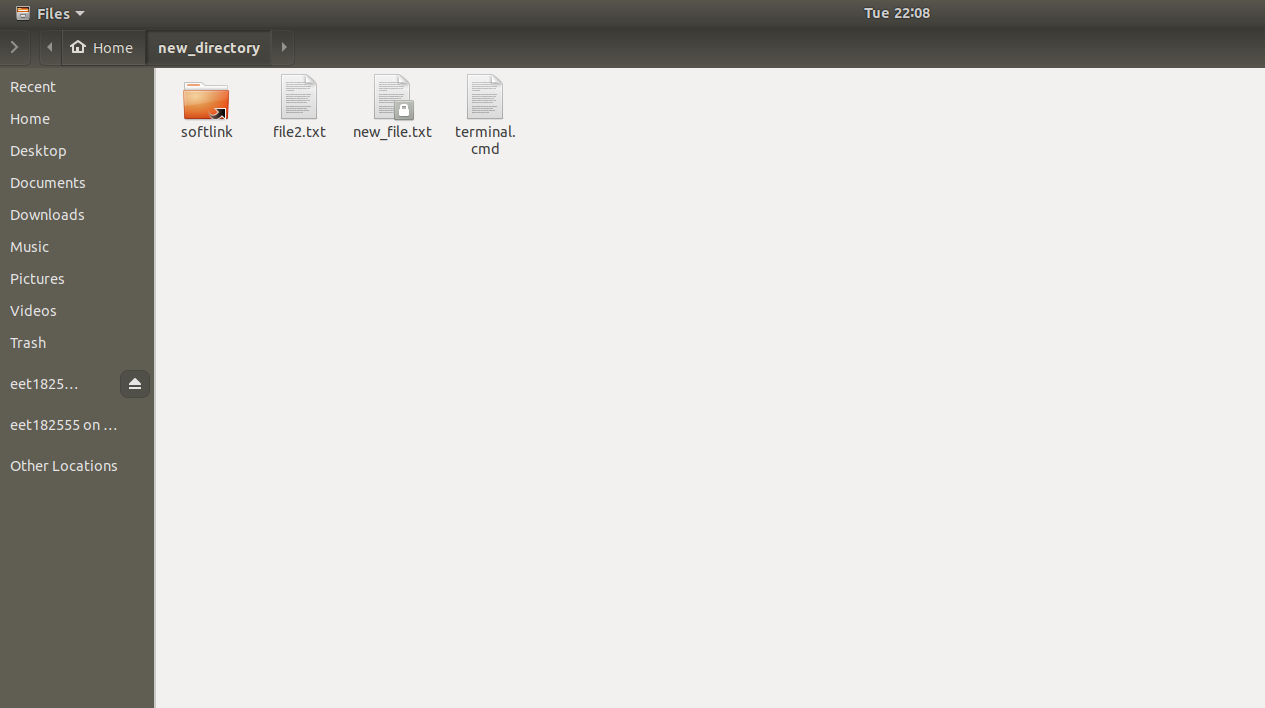
\includegraphics[scale=.3]{direc.png}
			\end{figure}

		
	
		\clearpage
	\section{Appendix}
		\subsection{Command History of Terminal}
		\begin{verbatim}
       27  ls
       28  cd
       29  pwd
       30  mkdir new_directory
       31  ls
       32  cd new_directory/
       33  pwd
       34  gedit new_file.txt
       35  chmod 444 new_file.txt 
       36  gedit new_file.txt 
       37  wc new_file.txt 
       38  gedit new_file.txt 
       39  grep -o "the" new_file.txt| wc -l
       40  echo "The world is round" >> new_file.txt 
       41  chmod 777 new_file.txt 
       42  echo "The world is round" >> new_file.txt 
       43  stat -c '%y' new_file.txt
       44  chmod 444 new_file.txt 
       45  stat -c '%y' new_file.txt
       46  touch -m new_file.txt 
       47  stat -c '%y' new_file.txt
       48  touch file2.txt
       49  ls
       50  sed -n '1,10p' new_file.txt >file2.txt 
       51  ln -s /home/abhaygupta/Documents softlink
       52  ls
       53  history> terminal.cmd
		\end{verbatim}
		\begin{thebibliography}{9}
\bibitem{ubuntu} 
Install ubantu along with wiindows,
\\\href{https://itsfoss.com/install-ubuntu-dual-boot-mode-windows/}{\texttt{https://itsfoss.com/install-ubuntu-dual-boot-mode-windows/}}
\bibitem{lc} 
linux commnds,
\\\href{https://www.howtogeek.com/412055/37-important-linux-commands-you-should-know/}{\texttt{https://www.howtogeek.com/412055/37-important-linux-commands-you-should-know/}}
\end{thebibliography}
\end{document}
